%!TEX root = ../dynamics.tex
\section{Market Analysis}
\label{sec:market}
Finally, we study the demand and supply of the Amazon MTurk marketplace. In the following, we define $Demand$ as the number of new tasks published on the platform by the requesters. In addition, we compute the average reward of the tasks that were posted. Conversely, we define $Supply$ as the workforce that the crowd is providing concretized as the number of tasks that got completed in a given time window by the workers. Again, we compute the average reward of the completed tasks.
In this section we use hourly collected data for the time period between June-October 2014.

\subsection{Supply vs. Demand}
First, we check whether supply and demand, in the context of Amazon MTurk marketplace, exhibit the standard behavior and relationship.
Figure \ref{fig:dsup} (right) shows the expected relationship between supply and price: The larger the supply, the lower the price evolves, which is the usual behavior in a market. On the other hand, Figure \ref{fig:dsup} (left) shows that the demand does not match the typical ascending demand curve (``the higher the demand the higher the price evolves''). Instead, the demand seems to be tied to the supply (i.e., the number of new HITs completed).

\begin{figure}[t!]
	\centering
		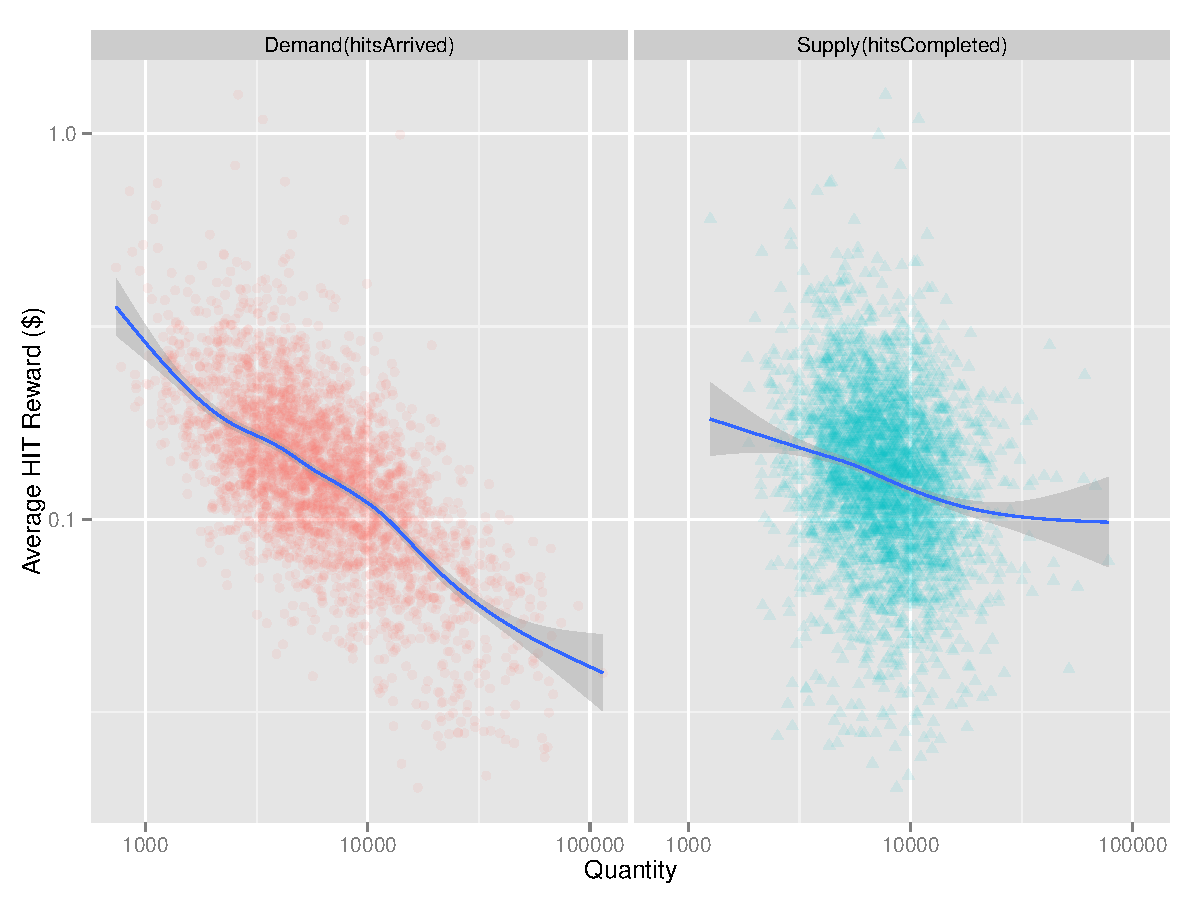
\includegraphics[width=0.48\textwidth]{figures/ds}
	\caption{The supply and demand for HITs versus the average HIT price.}
	\label{fig:dsup}
\end{figure}

\subsection{Supply Attracts new Workers} %

Now, we examine how the supply attracts new workers. First, we compare the three following variables: number of HITs published on the platform, number of HITs completed, and the average reward per HIT of both published and completed tasks. The results are depicted in Figure \ref{fig:scatter_matrix}. The apparent correlation between the rewards of the HITs completed and those published, and also among their quantities, gives us a first intuition that the crowd workers are sensitive to newly posted tasks, especially for those with higher prices.

\begin{figure}[t!]
	\centering
		
\includegraphics[width=0.48\textwidth]{figures/scatter}
	\caption{Scatter matrix comparing the different parameters in the demand and supply.}
	\label{fig:scatter_matrix}
\end{figure}

Next, we  analyze how the market reacts when new tasks arrive in the
market, to understand whether there is elasticity of supply. If the
supply of work is inelastic, the amount of work done over time should
be independent of the demand for work. So, if the amount of tasks
available in the market (``demand'') increases, then the percentage of
work that gets completed in the market should drop, as the same of
amount of ``work done" gets split among higher number of tasks. To
understand the elasticity of supply, we regressed the percentage of
work done in every time period (measured as the percentage of HITs
that are completed) against the number of new HITs that are posted in
that period. Figure \ref{fig:perc_hits_completed} shows the scatterplot for these two variables.

Our data reveals that an increase in the number of arrived HITs is
positively associated with a higher percentage of completed HITs. This
result provides evidence that the new work that is posted is more
attractive than the tasks previously available in the market, and attracts ``new
work supply".\footnote{Whether the supply comes from more distinct
workers, from workers that were idle, or from increased productivity
of existing workers is not possible to tell from our data.}

Our regression\footnote{Ordinary Least Squares (OLS)} of the ``Percent Completed" against ``Hits Arrived (in
1000's)", indicates an intercept of 2.5 and a slope of 0.05. To put
these numbers in context: On average, in the market there are 300K
HITs available, at any given time, and on average 10K new HITs arrive
every hour. The intercept of 2.5 means that 2.5\% of these 300K HITs
(i.e., 7.5K per hour) get completed, as a baseline, assuming that no
new HITs get posted. The slope is 0.05, meaning that if 10K new HITs
arrive within an hour, then the completion percentage increases by
0.5\%, to 3\% (i.e., 9K HITs per hour). When 50K new HITs arrive within
an hour, then the completion percentage increases to 5\% indicating
that 15K to 20K HITs get completed. In other words, approximately 20\%
of the \emph{new} demand gets completed within an hour of being posted,
indicating that new work has almost 10x higher attractiveness for the
workers than the work that is available on the website.
% 
This result could be explained by how tasks are presented to workers by \amt{}.
Workers, when not searching for tasks using specific keywords, are presented with the most recently published tasks first.

\begin{figure}[t!]
	\centering
	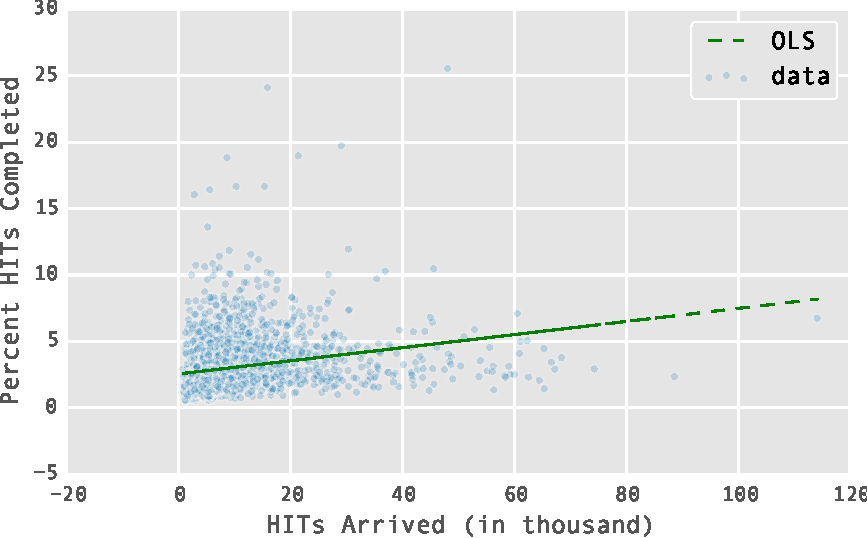
\includegraphics[width=0.48\textwidth]{figures/percent.pdf}
	\caption{The effect of new arrived HITs on the work  supplied.}
	\label{fig:perc_hits_completed}
\end{figure}

\subsection{Demand and Supply Periodicity}
On the demand side, we often observe some requesters frequently posting new batches of recurrent tasks. Hence, we are interested in the periodicity of such demand in the marketplace and the supply it drives. For that, we consider both the time-series of available HITs and the rewards completed over the period of three months. 

First, we observe that the demand exhibits a strong weekly periodicity, which is reflected by the autocorrelation that we compute the number of available HITs on Amazon Mturk (See Figure \ref{fig:hitav} and \ref{fig:achitav}). The market seems to have a significant memory that lasts for approximately 7-10 days.

Conversely, and to check for periodicity in the supply, we compute an autocorrelation on the weekly moving average convergence of the reward attached to completed HITs. Figure \ref{fig:mac} and \ref{fig:acmac} shows that there is a strong weekly periodicity effect as we observe high values in the range 0-250 hours.

\begin{figure*}[t!]
    \centering
    \begin{subfigure}[b]{0.48\textwidth}
        \centering
        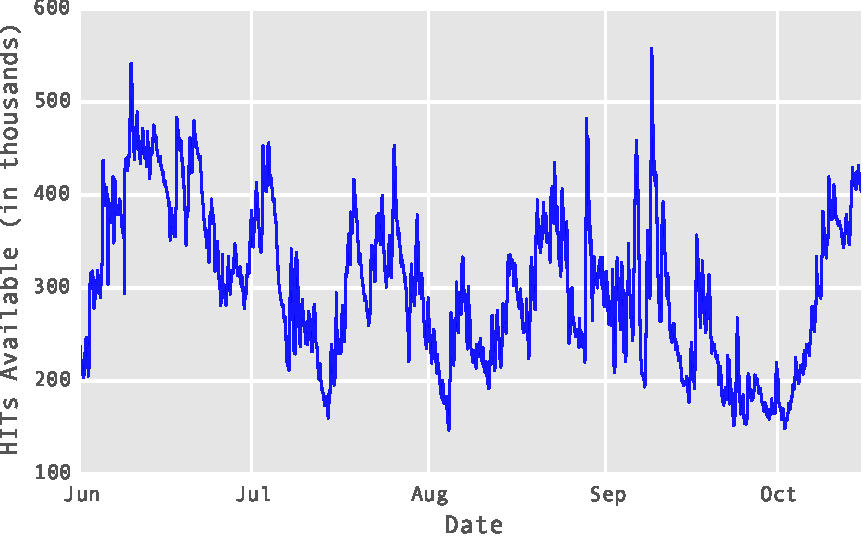
\includegraphics[width=\textwidth]{figures/out}
        \caption{HITs Available.}
        \label{fig:hitav}
    \end{subfigure}
    \hfill
    \begin{subfigure}[b]{0.48\textwidth}
        \centering
        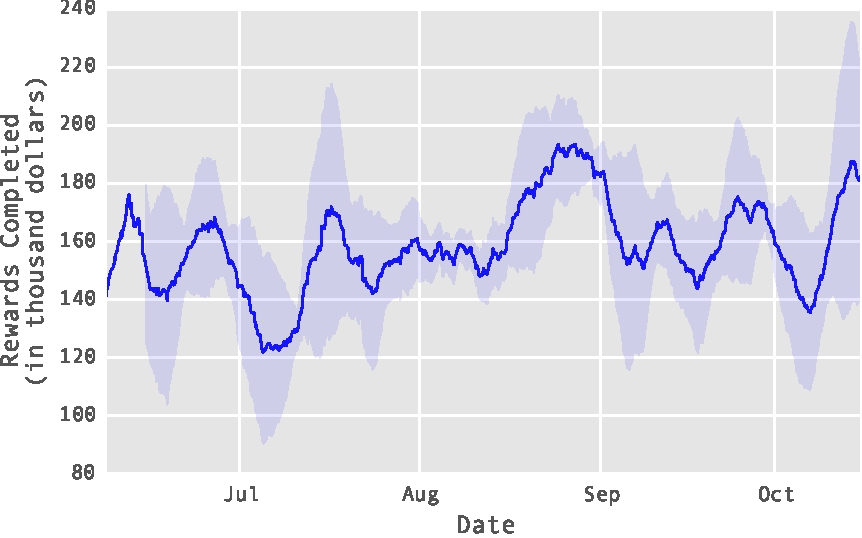
\includegraphics[width=\textwidth]{figures/mac}
        \caption{Weekly moving average on rewards completed.}
        \label{fig:mac}
    \end{subfigure}
    \hfill
    \begin{subfigure}[b]{0.48\textwidth}
        \centering
        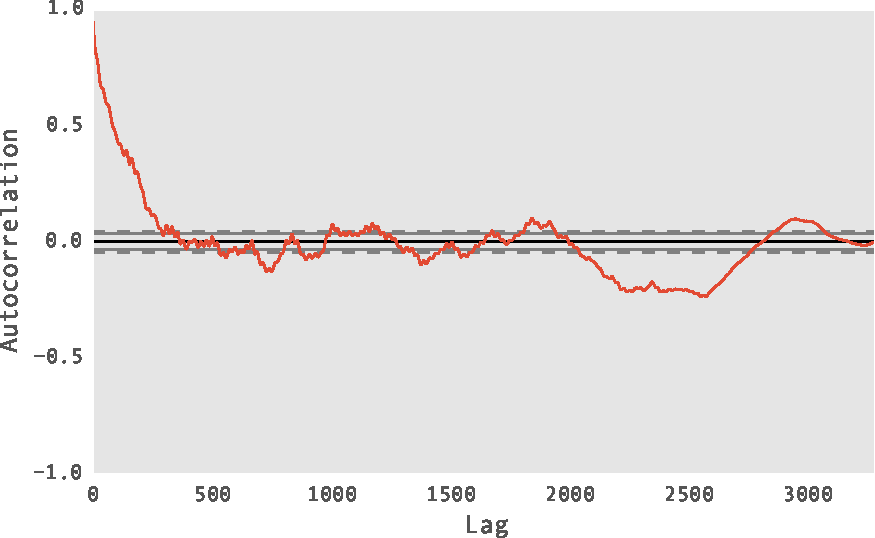
\includegraphics[width=\textwidth]{figures/out1}
        \caption{Autocorrelation on HITs available.}
        \label{fig:achitav}
    \end{subfigure}
    \hfill
    \begin{subfigure}[b]{0.48\textwidth}
        \centering
        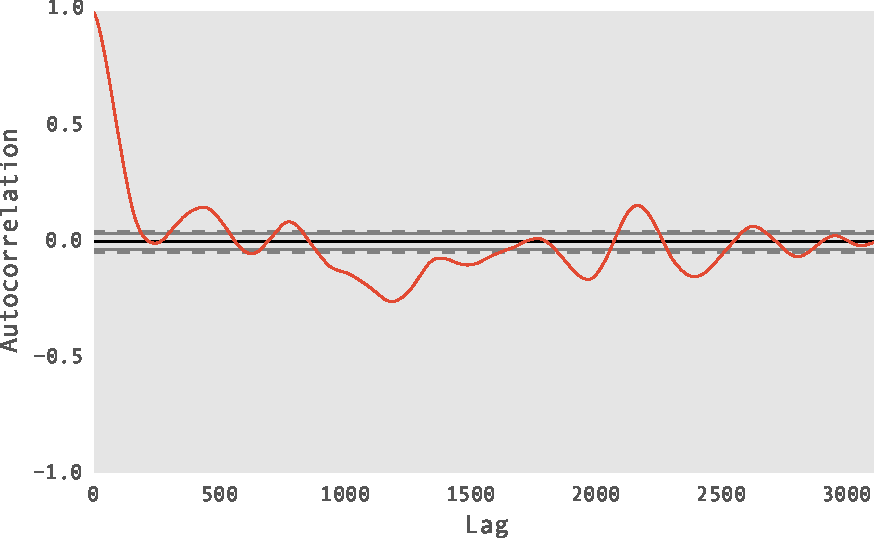
\includegraphics[width=\textwidth]{figures/macac}
        \caption{Autocorrelation on moving average of rewards completed.}
        \label{fig:acmac}
    \end{subfigure}
       
	\caption{Computed autocorrelation on the number of HITs available and on the weekly moving average of the completed reward (N.B., autocorrelation's Lag is computed in Hours). In both cases, we clearly see a weekly periodicity (0-250 Hours).}
	\label{fig:autocorrelation2}
\end{figure*}
